\documentclass[12pt]{article}

% preamble
\usepackage{amsmath}
\usepackage[margin = 1in]{geometry}
\usepackage{graphicx}
\usepackage{booktabs}
\usepackage{natbib}
\usepackage{multirow}
\usepackage{multicol}
\usepackage{setspace}
\usepackage{array}
\usepackage{pifont}
\usepackage[T1]{fontenc}
\usepackage[latin9]{inputenc}
\usepackage{babel}
\usepackage[table]{xcolor}
\usepackage{collcell}
\usepackage{hhline}
\usepackage{pgf}

% highlighting hyper links
\usepackage[colorlinks=true, citecolor=blue]{hyperref}

\title{Comparison of Multi-Class Classification Methods}
\author{Sean Murphy\\
  Statistics Major\\
  University of Connecticut
}

\doublespacing

% preparing for the confusion matrix table
\def\colorModel{hsb} 
\newcommand\ColCell[1]{
  \pgfmathparse{#1<50?1:0} 
    \ifnum\pgfmathresult=0\relax\color{white}\fi
  \pgfmathsetmacro\compA{0}
  \pgfmathsetmacro\compB{#1/55}
  \pgfmathsetmacro\compC{1}
  \edef\x{\noexpand\centering\noexpand\cellcolor[\colorModel]{\compA,\compB,\compC}}\x #1
  } 
\newcolumntype{E}{>{\collectcell\ColCell}m{0.4cm}<{\endcollectcell}}  %Cell width
\newcommand*\rot{\rotatebox{90}}

\begin{document}
\maketitle

\begin{abstract}

Classification tasks are a central facet of data science in our modern world.  
There are a multiplicity of viable classification techniques in use, and there 
are more being developed or simply improved all the time.  It is a natural 
question to investigate which methods are best suited to the task in which 
contexts, and there is already existing literature delving into these 
comparisons (\citet{alsafy2014multiclass}, \citet{khan2023comparison}, 
\citet{szollHosi2012comparison}).  This paper performs a comparative analysis 
of four different classification methods for multi-class classification: 
linear discriminant analysis, naive Bayes, K-nearest neighbors, and random 
forests. These models are fitted to a dataset containing physiochemical 
measurements on red wine samples from northern Portugal, in order to predict 
the quality of the wine.  Once the models were fitted to the dataset, it was 
clear that the random forest model outperformed the other models in terms of 
its predictive accuracy.  Thus, it is to be preferred to the other methods for 
modeling this dataset, and ought to be considered highly for multi-class 
classification tasks in general.  

\end{abstract}

\section{Introduction}
\label{sec:intro}

One central facet of the data science/machine learning world is the ability 
of researchers to design models that will accurately predict outcomes based 
on data.  Indeed, this is one of the major functions that data scientists 
play in the commercial world, academia, and elsewhere.  There is a tremendous 
demand, especially with the gargantuan quantities of data that are now at our 
disposal, for data scientists who can build effective models to learn from 
data and make accurate predictions for the future.

In general, prediction tasks can be of two types, depending on the characteristics 
of the response variable.  When the variable of interest is a numeric quantity, 
then the prediction task is termed \textit{regression}.  When the variable of 
interest takes different classes, however, the prediction task is termed 
\textit{classification}.  In classification, the goal of the researcher is to build 
a model that learns effectively from the input variables, the \textit{predictors}, 
and spits out accurate predictions of the class that should be assigned for a given 
vector of predictors, $x$.  The researcher considers various different models with 
their own respective strengths and weaknesses, and compares their relative 
performance to select the strongest one. 

Within classification, there are also two distinct types.  The simplest form of 
classification is \textit{binary classification}.  This is the circumstance in which 
the response variable only takes one of two classes, and the task is to predict which 
of these classes a given observation will take.  However, a response variable can take 
more than two classes.  This form of classification is known as 
\textit{multi-class classification}, and results in more complex models.

As there are both many different classification models and many different metrics for 
evaluating the effectiveness of classification models, there has been much literature 
comparing these methods.  Since the classification models all make different underlying 
assumptions, and since they have different relative strengths in different circumstances, 
it is a common practice to compare the performance of these methods on different datasets.  
Comparisons of multi-class classification methods have been carried out by 
\citep{alsafy2014multiclass}, \citep{khan2023comparison}, and \citep{szollHosi2012comparison}.  
Additionally, there are papers such as \citep{grandini2020metrics} and 
\citep{grandini2020metrics} that compare the utility of different classification metrics, 
depending upon the dataset and its associated characteristics.  

This paper will follow a similar vein of exploring various multi-class classification methods 
by a comparative analysis.  The analysis will focus on a dataset containing information on a 
collection of 1,599 red wine samples from northern Portugal.  The goal will be to predict the 
wine quality from a choice of 11 predictors, all of which are numeric physiochemical 
measurements of the wine samples.  I will fit a series of different multi-class classification 
models to the data, and will comparatively evaluate their performance.  From this analysis I 
hope to deduce which particular features of the dataset make it suitable for the classification 
method that proves the best.  I also aim to give an account of why the poorer-performing 
methods failed to provide relatively accurate predictions for the red wine quality.  

The rest of the paper will be organized in the following way.  An introduction to the red wine 
data set will be presented in Section~\ref{sec:data}.  This section will describe the variables 
and observations contained in the dataset, and will include a brief overview of summary 
statistics.  Next, a methodological overview of this analysis will be given in 
Section~\ref{sec:meth}.  Each of the classification methods and their underlying assumptions 
will be presented in Section~\ref{sec:class}.  The classification metric which will be used to 
compare the predictive effectiveness of each model will be introduced in Section~\ref{sec:metr}.  
After this, the results will be presented with tables and figures in Section~\ref{sec:resu}.  
Finally, once the results of the analysis have been described, a discussion of their 
implications and suggestions for further study will be covered in Section~\ref{sec:disc}.

\section{Data}
\label{sec:data}

The data that will be analyzed in this study comes from the UC Irvine Machine Learning 
Repository.  It is a dataset from 2009 containing information about a sample of red 
"Vinho Verde" wine from north Portugal.  The dataset contains $n = 1,599$ observations 
(different wine samples) of twelve variables, eleven of which are continuous numeric 
variables.  These continuous variables are different physiochemical measurements of the 
wine samples: fixed acidity, volatile acidity, citric acid, residual sugar, chlorides, 
free sulfur dioxide, total sulfur dioxide, density, pH, sulfates and alcohol.  The other 
variable contained in the dataset is wine quality, which takes integer values from 0-10 
(0 being lowest quality, 10 being highest quality).  Though numeric, this variable will 
be treated as having 11 classes, and will be the response variable in the analysis.  The 
goal is to predict the class of wine quality for a given sample of red wine based on its 
physiochemical properties.  

One important note before describing the methodology of this study concerns the response 
variable, wine quality.  A boxplot and histogram of the distribution of observations 
according to their wine quality levels can be seen in Figure~\ref{fig:wine}.  We can see 
that there are no wine samples in our dataset that had quality levels of 0, 1, 2, 9, or 
10.  All of the quality levels fell within the range from 3 to 8, and within this range, 
the vast majority were rated either a 5 or a 6.  Indeed, these two levels alone account 
for over 82 percent of the data.  We can see in the histogram and boxplot in 
Figure~\ref{fig:wine} that the distribution of wine quality levels is roughly symmetric, 
with outliers depicted in the boxplot at quality levels of 3 and 8.  Thus, the response 
variable has unbalanced classes; there are far from an equal number of observations in 
each class, especially considering that some classes do not contain any observations.  
The models built in this analysis will consequently ignore the missing classes for which 
there are no training observations.  

\begin{figure}[tbp]
 \centering
 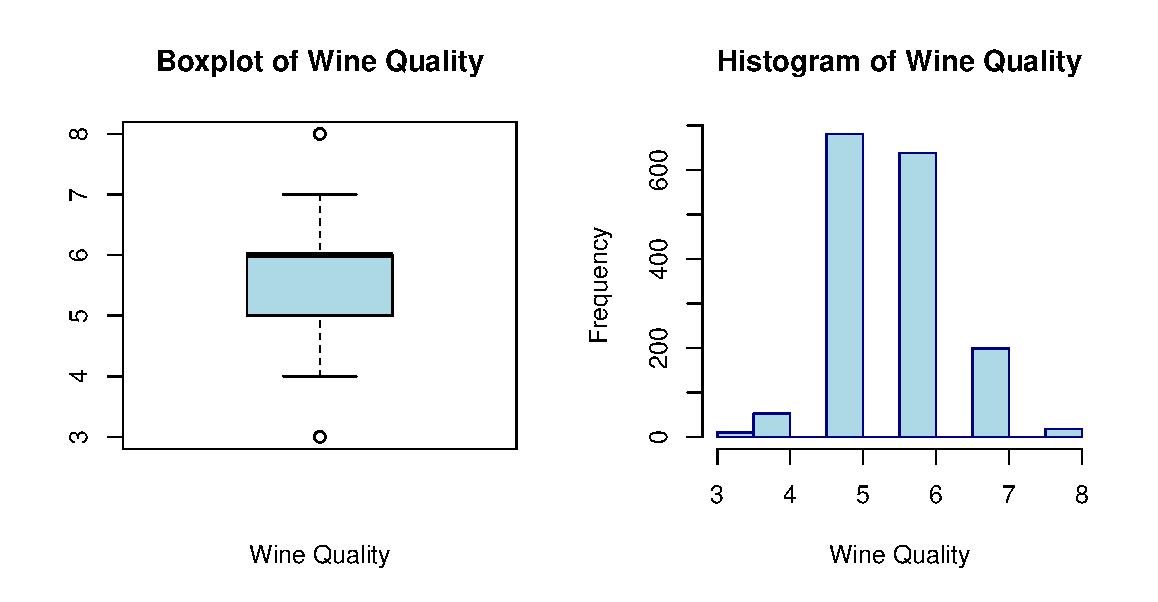
\includegraphics[width=\textwidth]{manuscriptfigure.pdf}
 \caption{A boxplot and a histogram of the wine quality for the samples of Portuguese red wine.}
 \label{fig:wine}
\end{figure}

\section{Methods}
\label{sec:meth}

Before proceeding straight into the analysis, it is necessary first to give an overview 
of the methodology that will be employed.  That means, first, summarizing how the data 
will be prepared, then introducing the models that will be used for this analysis.  
Finally, this section will also introduce the various metrics that will be used to evaluate 
model performance and to select the best classification method for the given dataset.  

\subsection{Data Preparation}
\label{sec:prep}

Fortunately, the red wine dataset is quite clean.  In the 1,599 rows of the data frame, there 
are no NA values, and thus no rows have to be removed.  

In order to be able to fit various models to the data set, we will first divide the dataset 
into a training and a test set.  The training set will comprise roughly three quarters of the 
dataset, and will be used to train the models, as the name would suggest.  Thus, it is from 
the data in the training set that the models will be constructed.  Observations from the red 
wine dataset will be assigned to the training set randomly, to avoid any kind of bias that 
would result from non-random training set selection.  

The remaining portion of the dataset will contain the test set.  The test set will be used 
to test the predictive accuracy of the models that were fitted using the training data.  
The fitted models will take as input the predictor values in the test set, and will spit 
out predictions for the response variable corresponding to each observation.  These 
classification predictions will then be compared to the observed response variable classes 
for each observation.  From this comparison, the overall accuracy of each model can be 
discerned, and they can be compared based on these findings.  The model that proves to 
perform the best will be the model that has the greatest overall prediction accuracy 
(equivalently the lowest overall test error), and this is the model that will be recommended 
for use. 

\subsection{Generative Models}
\label{sec:gm}

The first two multi-class classification methods are very similar in structure, and so it 
will be useful to introduce their shared underlying methodology before discussing their 
peculiarities.  This shared methodology is to employ Bayes' Theorem to obtain 
$Pr( Y = k | X = x)$ the probability that $Y$ falls into a particular class $k$ given a 
vector of predictors $x$ \citep{james2021introduction}.  Bayes' Theorem enables one to 
obtain $Pr( Y = k | X = x)$ indirectly by first obtaining the conditional distribution 
of $X$ in each class, $k$, and then using these distributions to obtain the desired 
probability that $Y$ will fall into $k$.  The general model takes the following form:
\begin{equation}
  \label{eq:genmod}
  Pr(Y = k | X = x) =
  \frac{\pi_k f_k(x)} {\sum_{l = 1} ^ {K} \pi_l f_l(x)}
\end{equation}
In Equation~\eqref{eq:genmod}, the $\pi_k$ term in the numerator simply is the prior 
probability that $Y$ falls into class $k$.  This is computed by the proportion of all 
the observations in the sample that fall into the $k ^ {th}$ class.  The $f_k(x)$ term 
describes the conditional distribution of $X$ in class $k$.  In other words, 
$f_k(x) = Pr(X = x | Y = k)$.  These two numerator terms are divided by the same two 
terms for each class $k$ summed in the denominator.  That is, the denominator contains 
the sum of the prior probabilities that $Y$ will fall into each of the $K$ classes 
multiplied by the corresponding conditional distribution of $X$ in that class.  Thus, 
the general form of the generative model is simply Bayes' Theorem, which returns here 
an estimate of the probability that $Y$ will fall into class $k$ given some vector of 
predictors.  

Each of the next two multi-class classification models that we will consider is some 
variant of the above, and they are principally differentiated by their varying strategies 
for approximating $f_k(x)$.  The two kinds of generative models that we will consider in 
this paper are linear discriminant analysis (LDA) and naive Bayes (NB).  We will discuss 
each of them in turn.  

\subsubsection{Linear Discriminant Analysis}
\label{sec:lda}

Linear Discriminant Analysis (LDA) is a generative model that approximates $f_k(x)$ by 
assuming that each of the predictors comes from a normal distribution.  In the case of 
multiple predictors such as we have in this analysis, this means that LDA assumes $x$ 
(the vector of $p$ predictors) follows a multivariate normal distribution.  The mean, 
$\mu$, of this multivariate normal distribution is a vector containing the mean value 
of each predictor.  The covariance of the predictors, $\Sigma$, is the $p$ by $p$ 
covariance matrix of the vector $x$.  Therefore, we can say in shorthand that 
$x \sim N(\mu,\Sigma)$.  Thus, since the conditional distribution of the vector $x$ in 
each class $k$ is assumed to be multivariate normal, the density function is 
$$Pr(X = x|Y = k) = \frac {1} {(2\pi) ^ {p/2} |\Sigma| ^ {1/2}} exp(-\frac{1}{2} 
(x - \mu_k) ^ T \Sigma ^ {-1} (x - \mu_k))$$ \citep{james2021introduction}.  Here, 
$\mu_k$ is simply the vector of the mean values of the $p$ predictors where $Y = k$, 
and $\Sigma$ is the common covariance matrix of $x$ for each of the $k$ classes.  The 
above equation can then be plugged into Equation~\eqref{eq:genmod} for $f_k(x)$, the 
resulting equation of which we will not reproduce here because of its complexity.  
Suffice it to say that this equation now obtains for us the probability that $Y$ falls 
in class $k$ given a particular vector of predictors $x$, so that the model gives the 
value for $Pr(Y = k|X = x)$.

In order to classify a vector of predictors $x$ to some class $Y = k$, we look for the 
class in which the value of the above $Pr(Y = k|X = x)$ is greatest.  With some algebraic 
rearrangement, this is equivalent to classifying a vector $x$ to the class for which the 
following equation is greatest:
\begin{equation}
  \label{eq:disscore}
  \delta_k(x) = x ^ T \Sigma ^ {-1} \mu_k - 
  \frac {1} {2} \mu_k ^ T \Sigma ^ {-1} \mu_k + \log {\pi_k}
\end{equation}. 

Equation~\eqref{eq:disscore} is called the \textit{discriminant score} 
\citep{james2021introduction}.  If a class has the greatest value of $\delta_k(x)$ for some 
vector of predictors $x$, then that vector of predictors will be classified to the corresponding 
class.  Linear discriminant analysis gets its name from the fact that this discriminant score is 
a linear function of $x$.

In Equation~\eqref{eq:disscore}, each $\mu_k$ is estimated by combining the mean value for each 
predictor in the sample into a vector, $\hat{\mu_k}$.  The values of $\pi_k$ are once again the 
prior probability that $Y$ falls into class $k$, calculated by the proportion of the total 
observations in class $k$.  Finally, the covariance matrix of the predictors, $\Sigma$, is 
estimated by finding the covariance matrix of the predictors in the sample.     

\subsubsection{Naive Bayes}
\label{sec:nb}

Naive Bayes (NB) is distinct from LDA in the manner it estimates $f_k(x)$, the conditional 
joint distribution of the $p$ predictors given that $Y$ is in some class $k$.  Whereas LDA 
assumes that this joint distribution is a multivariate normal distribution, NB assumes that 
each of the $p$ predictors are independent within each class \citep{james2021introduction}.  
Thus, for a particular class, the joint probability distribution of all the predictors given 
that $Y$ falls in that class is simply a product of the individual densities of each of the 
predictors given $Y = k$.  In more formal terms, because of this assumption of the independence 
of each predictor within each class, NB estimates $f_k(x)$ in the following manner:
\begin{equation}
  \label{eq:indprob}
  f_k(x) = f_{k1}(x_1) \times f_{k2}(x_2) \times ... \times f_{kp}(x_p)
\end{equation} 
where $k = 1, 2, ..., K$, and $x_1, x_2, ..., x_p$ are the $p$ predictors in the training set.  
Thus, Equation~\eqref{eq:indprob} can simply be plugged into Equation~\eqref{eq:genmod} for 
$f_k(x)$ in the following manner:
\begin{equation}
  \label{eq:nb}
   Pr(Y = k | X = x) =
  \frac{\pi_k [f_{k1}(x_1) \times f_{k2}(x_2) \times ... \times f_{kp}(x_p)]} 
  {\sum_{l = 1} ^ {K} \pi_l [f_{l1}(x_1) \times f_{l2}(x_2) \times ... \times f_{lp}(x_p)]}
\end{equation} 
where $k = 1, 2, ..., K$.  The $f_{kp}(x_p)$ terms in Equation~\eqref{eq:nb} are much simpler 
to estimate than the joint distribution of each of the predictors, so NB simplifies the 
analysis greatly.  Though there are many strategies for estimating these individual predictor 
densities within each class, these strategies will not be covered within this paper.  

Although NB makes a strong (and often in practice, untrue) assumption about the independence 
of the predictors, it still performs quite well in many circumstances.  It is particularly 
well suited to situations in which the training set is not large enough relative to the number 
of predictors to effectively estimate the joint density of each of the predictors.  

\subsubsection{K-Nearest Neighbors}
\label{sec:knn}

The K Nearest Neighbors (KNN) approach to multi-class classification is markedly different 
from those covered previously.  It has a rather intuitive design, and its methodology is 
rather straightforward.  Interestingly enough, it also often obtains usefully low test error 
rates and can perform quite well on many data sets.  

Up until now, $K$ has signified the number of distinct classes that can be taken by $Y$, the 
response variable of interest.  In KNN, K refers to the number of nearest neighbors upon 
which the classification prediction is based.  To forestall further confusion, therefore, 
$K$ will still be used to denote the number of classes taken by $Y$, while $K ^ *$ will refer 
to the number of nearest neighbors in KNN analysis.  

The basic idea behind KNN is that, if we wish to accurately predict which class $Y$ will fall 
into given some vector of predictors $x$, we ought simply to look at the classes taken by $Y$ 
given vectors as similar to $x$ as we can find in our dataset.  In practical terms, this means 
that we base our prediction of $Y$'s class upon the class taken by the largest number of the 
$K ^ *$ nearest neighbors to $x$.  The $K ^ *$ nearest neighbor observations to $x$ are the 
observations with the shortest Euclidean distance to the vector $x$.  The value of $K ^ *$ can 
be adjusted by the researcher when fitting KNN models, since different values of $K ^ *$ will 
perform better under different scenarios.  Thus, one can fit many different KNN models to the 
same dataset, each with different numbers of nearest neighbors, to predict the class of $Y$ 
for some vector of predictors, $x$.  

One notable drawback of KNN analysis is its decreased accuracy as the number of predictors 
increases.  Holding all other things constant, when the number of predictors increases, the 
Euclidean distance between the vector $x$ of interest and each of its $K ^ *$ nearest neighbors 
also increases.  As such, the nearest neighbors to $x$ provide decreasingly satisfactory 
approximations of $x$, and thus KNN models fitted in high dimensions (i.e., with many 
predictors) tend to have poorer performance in terms of prediction accuracy and test errors.  
This pattern is known as the \textit{curse of dimensionality}, and is an important reason to 
be wary in instances of large values of $p$.  We must keep this in mind given that, for our 
current analysis, $p = 11$. 

\subsection{Tree-Based Methods}
\label{sec:tbm}

Tree-based methods are another popular strategy for modeling data.  Tree-based methods can be 
applied both for regression and classification tasks.  The most basic form of such a method is 
the simple decision tree.  Decision trees work by partitioning the predictor space into $m$ 
distinct and non-overlapping regions, $R_1, ... , R_m$, and then predicting at some uniform 
value for each observation within that region.  For regression tasks, a vector of predictors 
$x$ in region $R_i$ is predicted to be the mean of the response values for all the observations 
in $R_i$.  For classification tasks, however, $x$ will be predicted to take the class that is 
taken by the most observations in $R_i$; it is a simple majority vote.  

Most of the computational work that is done in generating simple decision trees comes when 
subdividing the predictor space.  This is done in a sequential process.  At each step, every 
possible binary split in the predictor space is considered as a candidate for the first branch 
of the tree overall.  These candidate split zones are compared against each other according to 
some metric which depends on the prediction task, and then the optimal split is chosen.  For 
regression tasks, the optimal split will be the one that yields the lowest overall residual 
sum of squares of the resulting model.  For classification tasks, there are two main metrics 
that are used for determining the optimal splitting point: the Gini index and the cross-entropy 
value.  The Gini index is calculated in the following way:

\begin{equation}
  \label{eq:gini}
   G = \sum_{k = 1} ^ {K} \hat{p}_{mk} (1 - \hat{p}_{mk}).
\end{equation} 

Essentially, the Gini index is derived from the formula for the variance of Bernoulli random 
variables.  The term $\hat{p}_{mk}$ in Equation~\eqref{eq:gini} is the proportion of 
observations in region $m$ that take on class $k$.  In the above equation, we see that 
$\hat{p}_{mk} (1 - \hat{p}_{mk})$ is minimized when $\hat{p}_{mk}$ is closest either to $0$ 
or to $1$, and is maximized when $\hat{p}_{mk} = 0.5$.  Thus, the Gini index is essentially 
a measure of the purity of each region, in terms of the proportion of observations within that 
region that take on one particular class.  When the Gini index is used, the tree will be split 
at the point that minimizes the Gini index.  

Cross-entropy is a very similar alternative to the Gini index.  Instead of being calculated 
using the formula for the variance of a Bernoulli random variable, it is calculated in the 
following manner:

\begin{equation}
  \label{eq:crossent}
   D = - \sum_{k = 1} ^ {K} \hat{p}_{mk} log (\hat{p}_{mk}).
\end{equation} 

Although the $log$ function is used in Equation~\eqref{eq:crossent}, the overall term behaves 
very similarly to the Gini index.  The negative sign in front of the summation is there to 
ensure that the goal is still to minimize this metric to select the optimal splitting point.  
Once the predictor space has been split, the same process is repeated to perform the other 
splits until the desired tree size has been reached.  This tree can then be used to predict 
the response for observations in the test set.  Although simple decision trees do not often 
outperform their competitors, there are more advanced tree-based methods that predict quite 
accurately.  

\subsubsection{Random Forests}
\label{sec:rf}

One such advanced tree-based method is the random forest (RF).  Random forest models employ 
two major techniques to enhance the prediction accuracy relative to simple decision trees.  
The first is to utilize the bootstrap.  In statistics, bootstrapping simply refers to taking 
repeated random samples without replacement from an original dataset in order to generate a 
pseudo-population.  Then, the estimate of the parameter of interest can simply be an average 
of all these $B$ bootstrapped datasets.  When this strategy is applied to trees, this means 
that for each bootstrapped sample, a separate tree is grown, 
$\hat{f} ^ {*b} (x)$.  The prediction for some observation, $x$, will then be the most 
frequently predicted class among all the trees for $x$.  

The second technique employed by RF models is the introduction of randomness in the 
tree-growing process itself.  One problem with trees grown on bootstrapped datasets is that 
they may have high correlations with each other.  RF models attempt to decorrelate the trees 
by only considering some subset, $s$, of the $p$ predictors to partition that data over at 
each splitting step.  Thus, at each step, a subset of $s$ predictors is randomly selected, 
and the tree will only branch along one of those predictors.  This strategy helps to reduce 
the variance of the model overall.  Although the value of $s$ can be selected in various 
manners, one common choice of $s$ is the integer closest to $\sqrt{p}$.

Thus, with these two strategies, random forests tend to improve drastically upon the 
foundation laid by simple decision trees.

\subsection{Classification Metrics}
\label{sec:metr}

Once the models have been constructed, the next task is to select the criteria by which 
their performance will be evaluated and compared.  Without going into an excessive degree 
of length, this section will present a brief overview of how a multi-class classification 
model's performance can be evaluated.

\subsubsection{Confusion Matrices}
\label{sec:cm}

% hypothetical confusion matrix example for a multi-class classfication model
\begin{table}[tbp]
\caption{This is a hypothetical example of a multi-class confusion matrix.}
\label{tab:conf}
\centering
\newcommand\items{5}   %Number of classes
\arrayrulecolor{gray}
\noindent\begin{tabular}{cc*{\items}{|E}|}
\multicolumn{1}{c}{} &\multicolumn{1}{c}{} &\multicolumn{\items}{c}{Actual} \\ \hhline{~*\items{|-}|}
\multicolumn{1}{c}{} & 
\multicolumn{1}{c}{} & 
\multicolumn{1}{c}{\rot{Class A}} & 
\multicolumn{1}{c}{\rot{Class B}} & 
\multicolumn{1}{c}{\rot{Class C}} & 
\multicolumn{1}{c}{\rot{Class D}} &
\multicolumn{1}{c}{\rot{Class E}} \\ \hhline{~*\items{|-}|}
\multirow{\items}{*}{\rotatebox{90}{Predicted}} 
&Class A  & 90 & 1  & 5 & 2 & 3 \\ \hhline{~*\items{|-}|}
&Class B  & 7 & 83  & 8 & 1 & 0 \\ \hhline{~*\items{|-}|}
&Class C  & 3 & 0  & 88 & 7 & 4 \\ \hhline{~*\items{|-}|}
&Class D  & 7 & 2 & 8 & 92 & 5 \\ \hhline{~*\items{|-}|}
&Class E  & 3 & 0 & 4 & 9 & 93 \\ \hhline{~*\items{|-}|}
\end{tabular}
\end{table}

A confusion matrix is a basic analytical tool for evaluating classification model performance.  

In the confusion matrix in Table~\ref{tab:conf}, the predicted classes are the rows and the 
actual (test dataset) classes are the columns.  The classes in both the rows and columns are 
presented in exactly the same order.  Thus, when the model predicts that a particular 
observation will take on a specific class, if that same observation took the predicted class 
in the test dataset, then the row and column values match.  This would be an instance of an 
observation that is correctly predicted by the model.  Thus, since the classes in the rows 
and columns are presented in the same order, the diagonal elements of the confusion matrix 
are the correctly predicted observations.  These are all the observations whose predicted 
class matches its actual class, and they are highlighted in Table~\ref{tab:conf}.  

On the other hand, all the elements of the confusion matrix that are not on the diagonal are 
the incorrectly predicted observations.  These are the observations whose predicted class 
does not match their actual class.  The calculations that follow are predicated on the 
presentation of correctly versus incorrectly predicted observations in the confusion matrix.  

\subsubsection{Classification Accuracy Value}
\label{sec:CAV}

The Classification Accuracy Value (CAV) is the simplest and most straightforward means of 
assessing the overall prediction accuracy of a classification model.  To calculate the CAV 
using a confusion matrix, simply sum the diagonal elements of the matrix in the numerator, 
and sum all the elements of the matrix in the denominator.  The corresponding proportion 
will be the proportion of observations whose class is predicted accurately by the model.  
This value is the Classification Accuracy Value.  The calculation for this metric is 
presented in Equation~\eqref{eq:cav}:
\begin{equation}
    \label{eq:cav}
    CAV = \frac {T} {T + F}
\end{equation}
, where $T$ stands for the true predictions (on the diagonal of the matrix) and $F$ stands 
for the false predictions, which are the non-diagonal elements.  

The CAV is best applied in situations where the overall prediction accuracy of the model 
is of the highest concern, and where class-specific prediction accuracy is less important.  
In terms of the CAV, each observation is equally weighted, but the relative prediction 
accuracy within each class is not taken as strictly into account as in other metrics, which 
we will not explore here.  If it is of the utmost importance that the model has a high 
prediction accuracy for each class, then other metrics may be applied that take this factor 
into account. 

\section{Results}
\label{sec:resu}

% table with the results
\begin{table}[]
    \centering
    \begin{tabular}{@{}lll@{}}
    \toprule
\textbf{Method} & \textbf{Specification} &\textbf{CAV} \\
\midrule
    KNN                          & \# of Neighbors  &          \\
                                 & 1  & 59.1\%   \\
                                 & 5  & 47.1\%   \\
                                 & 15 & 51.6\%   \\ \midrule
    LDA      &    & 63.7\%   \\ \midrule
    NB       &    & 55.4\%   \\ \midrule
    RF &    & 69.7\%   \\ \bottomrule
    \end{tabular}
    \caption{Classification Accuracy Value for each classification method.}
    \label{tab:results_table}
    \end{table}

% bar chart depicting the results
\begin{figure}[tbp]
 \centering
 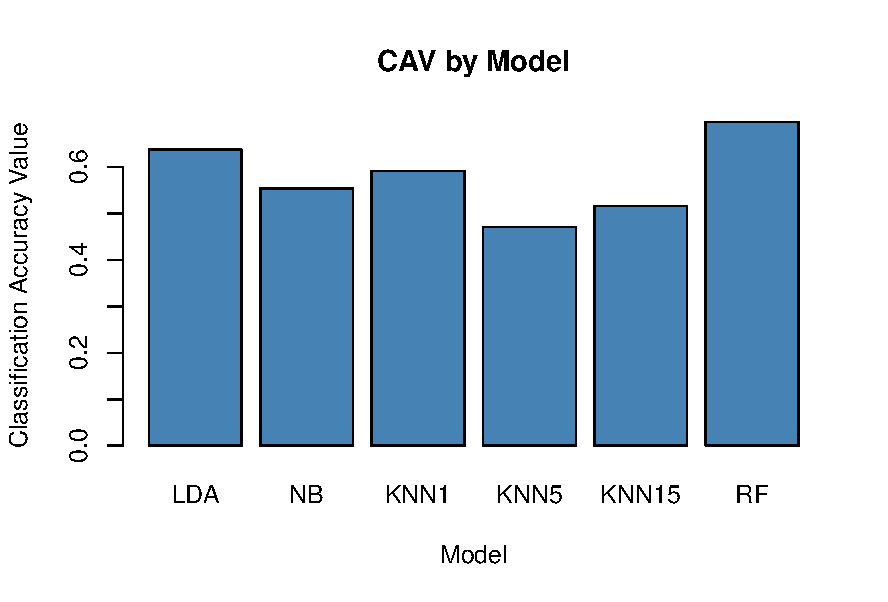
\includegraphics[width=\textwidth]{model_performance_figure.pdf}
 \caption{A bar chart with the Classification Accuracy Value for each model.}
 \label{fig:performance}
\end{figure}

We can see from both Table~\ref{tab:results_table} and Figure~\ref{fig:performance} that 
the random forest method is the clear favorite amongst all the models that have been explored 
in this analysis.  Its Classification Accuracy Value of $69.7\%$ is much higher than most of 
the other models, with the closest competitor being the LDA model at $63.7\%$.  This not a 
particularly surprising result, as random forest models generally have greater complexity 
and often outcompete their classification competitors.  While complexity itself does not 
necessarily entail enhanced accuracy on test sets, the RF model here seems to have the 
complexity required to match that of the data itself.  The simpler methods with more basic 
assumptions, such at the KNN models and the NB model, seem to have seriously underperformed.  
While it can be difficult to interpret random forest models in comparison to, say, KNN models, 
their predictive power often is sufficient to recommend them for use.  Thus, for predicting 
the quality of red wine samples, the RF model is selected above the other models.  

\section{Discussion}
\label{sec:disc}

With the emergence of both new classification methods and new improvements on existing methods 
occurring with relative frequency in recent decades, there have been a flurry of papers 
attempting to perform comparative analyses, such as in \citep{alsafy2014multiclass}, 
\citep{khan2023comparison}, and \citep{szollHosi2012comparison}.  As is often seen, the 
performance of a given method can be highly variable depending upon the dataset that trains 
it and the dataset that it is tested on.  For a model to perform well, its particular 
qualities -- its particular strengths, must be realized by the dataset.  Thus, when a model 
like LDA assumes that the predictors within each class follow a multivariate Gaussian 
distribution, the LDA model will perform well when this assumption is closest to being true 
in the data that it is trained and tested on.  When this assumption is clearly violated, the 
LDA model will struggle.  Thus, it is useful to compare classification methods across a 
variety of dataset types to gain a more complete understanding of the contexts in which 
particular methods tend to excel.  

This particular study, due to the constraints of space, was not able to delve more deeply 
into the various classification metrics that have been developed to assess model performance.  
The literature is rich and gradually expanding in this area, and it would be quite interesting 
to evaluate these models in more depth.  Using different, more complicated metrics would enable 
us to develop a clearer understanding of the respective strengths and weaknesses of each model.

Future studies, thus, should continue to address classification metrics, and the particular 
insights they provide into a comprehensive analysis of model performance.  Moreover, there is 
always a need to spend more time and effort developing new models, and tweaking current models 
to optimize their predictive power.  This is an exciting field that is full of potential for 
innovation, and it will be fascinating to watch it continue to evolve over the course of the 
next few decades. 

\bibliography{references}
\bibliographystyle{chicago}

\end{document}